%% hack to load amsfonts instead of amssymb to properly make hbar bold
\RequirePackage{scrlfile}
\makeatletter
\AfterPackage{beamerbasemodes}{\beamer@amssymbfalse}
\makeatother
\documentclass[xcolor={svgnames,rgb}]{beamer}
\let\oldhbar\hbar
\usepackage{amssymb}
\def\hbar{\boldsymbol{\oldhbar}}

%%other packages
\usepackage{braket}

%% fonts

\usepackage[no-math]{fontspec}
%\setmainfont[Mapping=tex-text,Numbers={Lining}]{Hoefler Text}
\setmainfont[Mapping=tex-text]{Optima}
\usepackage[SlantFont]{xeCJK}
%\setCJKmainfont{Hiragino Maru Gothic Pro}
\setCJKmainfont{Hiragino Mincho Pro}
%\setCJKmainfont{Hiragino Sans W2}
\setCJKfamilyfont{tt}{Hiragino Maru Gothic Pro}




%% colors

\definecolor{myblue}{HTML}{100080}
\definecolor{math}{HTML}{100080}
\definecolor{blendedblue}{rgb}{0.2,0.2,0.7}

\def\bff{\ifmmode\else\bfseries\fi}
\def\black#1{\textcolor{Black}{#1}}
\def\red#1{\textcolor{Crimson}{\bff #1}}
\def\green#1{\textcolor{ForestGreen}{\bff #1}}
\def\blue#1{\textcolor{myblue}{\bff #1}}
\def\orange#1{\textcolor{Orange}{\bff #1}}
\def\purple#1{\textcolor{Purple}{\bff #1}}
\def\alert#1{\red{#1}}

\everymath{\displaystyle\color{math}}
\let\olddisplaystyle\displaystyle
\def\displaystyle{\olddisplaystyle\color{math}}
\let\oldbracket\[
\def\[{\oldbracket\color{math}}



%% hyperref setup
%\hypersetup{colorlinks=true,urlcolor=Purple}
\let\oldhref\href
%\def\href#1#2{\oldhref{#1}{\purple{#2}}}


%% citation etc
\def\loosecite#1{\textcolor{Purple}{[#1]}}
\def\arxiv#1{\oldhref{http://arxiv.org/abs/#1}{#1}}
\long\def\openquestion#1{%
\begin{block}{Open question}
#1
\end{block}
}



%% beamer setup
\usetheme{Boadilla}
\usecolortheme{default}
\usecolortheme[named=Crimson]{structure}
\setbeamercolor{frametitle}{fg=ForestGreen}
\setbeamercolor{titlelike}{bg=white}
\setbeamercolor{palette primary}{bg=white!70}
\setbeamercolor{palette secondary}{bg=white!80}
\setbeamercolor{palette tertiary}{bg=white!90}
\setbeamercolor{palette quaternary}{bg=white}
\setbeamercolor{button}{use=local structure,fg=local structure.fg!80!bg,bg=white}
\setbeamercolor{button border}{use=local structure,fg=local structure.fg!80!bg}

\usefonttheme{serif}
\usefonttheme{professionalfonts}
\setbeamerfont{structure}{series=\bfseries}
\setbeamerfont{subsection in toc}{parent=section in toc}

\setbeamertemplate{items}[circle]
\setbeamertemplate{sections/subsections in toc}[sections numbered]
\setbeamertemplate{navigation symbols}{} 


\setbeamertemplate{footline}
{
\leavevmode%
\hbox{%
	\begin{beamercolorbox}[wd=.333333\paperwidth,ht=2.25ex,dp=1ex,center]{author in head/foot}%
	\usebeamerfont{author in head/foot}  \end{beamercolorbox}%
	\begin{beamercolorbox}[wd=.333333\paperwidth,ht=2.25ex,dp=1ex,center]{title in head/foot}%
		\usebeamerfont{title in head/foot}\insertshorttitle
	\end{beamercolorbox}%
	\begin{beamercolorbox}[wd=.333333\paperwidth,ht=2.25ex,dp=1ex,right]{date in head/foot}%
		\usebeamerfont{date in head/foot}\insertshortdate{}\hspace*{2em}%
		\insertframenumber{} / 55 %\inserttotalframenumber %
		\hspace*{2ex}%
	\end{beamercolorbox}}%
	\vskip0pt%
}

\let\frametitleoriginal\frametitle
\def\frametitle#1{\frametitleoriginal{#1\vphantom{Hpgy}}}



%% other misc macros
\def\slash#1{\ooalign{\hfil\big/\hfil\crcr$#1$}}
\def\tr{\mathop{\mathrm{tr}}\nolimits}

\def\cL{\mathcal{L}}
\def\bQ{\mathbb{Q}}
\def\bR{\mathbb{R}}
\def\bC{\mathbb{C}}
\def\bZ{\mathbb{Z}}
\def\cN{\mathcal{N}}
\def\cD{\mathcal{D}}
\def\cA{\mathcal{A}}
\def\cF{\mathcal{F}}
\def\cH{\mathcal{H}}
\def\cO{\mathcal{O}}
\def\cS{\mathcal{S}}
\def\cV{\mathcal{V}}
\def\cP{\mathcal{P}}
\def\cM{\mathcal{M}}

\def\vev#1{\langle#1\rangle}
\def\vol{\mathop{\mathrm{vol}}\nolimits}
\def\diag{\mathrm{diag}}
\def\triv{\mathrm{triv}}
\def\SCFT{\mathrm{SCFT}}
\def\Spin{\mathrm{Spin}}
\def\Pin{\mathrm{Pin}}
\def\U{\mathrm{U}}
\def\SU{\mathrm{SU}}
\def\SL{\mathrm{SL}}
\def\SO{\mathrm{SO}}
\def\O{\mathrm{O}}
\def\USp{\mathrm{USp}}
\def\Sp{\mathrm{Sp}}
\def\u{\mathfrak{u}}
\def\su{\mathfrak{su}}
\def\so{\mathfrak{so}}
\def\usp{\mathfrak{usp}}
\def\sp{\mathfrak{sp}}
\def\hkq{/\!/\!/}
\def\RP{\mathbb{RP}}

\def\Nequals#1{$\mathcal{N}{=}#1$}


\subject{Unoriented}
\date[]{}

\usepackage{tikz}
\usepackage{pbox}

\begin{document}

\parskip1em 
\boldmath
\def\baselinestretch{1.1}



\def\incb#1{\vcenter{\hbox{\includegraphics[scale=.18]{#1}}}}
\def\inc#1{\vcenter{\hbox{\includegraphics[scale=.15]{#1}}}}
\def\incx#1{\vcenter{\hbox{\includegraphics[scale=.4]{#1}}}}
\def\incc#1{\vcenter{\hbox{\includegraphics[scale=.12]{#1}}}}


{%
\setbeamercolor{background canvas}{bg=myblue!70!black}
\setbeamercolor{author in head/foot}{fg=white, bg=myblue!70!black}
\setbeamercolor{title in head/foot}{fg=white, bg=myblue!70!black}
\setbeamercolor{date in head/foot}{fg=white, bg=myblue!70!black}
\begin{frame}
\vbox{}
\vfill
%\begin{exampleblock}{}
\begin{center}
\bfseries\huge\color{White} Anomaly of electromagnetic duality \\
of the Maxwell theory

\bigskip\bigskip\bigskip

\large Yuji Tachikawa (立川裕二)

{based on my work with} \\
{Chang-Tse Hsieh (謝長澤) \& Kazuya Yonekura (米倉和也)}

\bigskip\bigskip

Topological Science Symposium 2019, Keio, Nov.~20
\end{center}
%\end{exampleblock}
\vfill
\vbox{}
\end{frame}
}

\if0
\begin{frame}
\bigskip\bigskip\bigskip\bigskip\bigskip

\vfill

%\rmfamily

\begin{exampleblock}{}
\begin{center}\LARGE\bfseries
\color{math}
Anomaly of electromagnetic duality \\
of the Maxwell theory
\end{center}
\end{exampleblock}

\bigskip\bigskip\bigskip
\begin{center}
\large  \blue{}


\bigskip
\large \alert{Topological Science Symposium 2019, Keio, Nov.~20}

\end{center}
\bigskip\bigskip\bigskip
\vfill


\end{frame}
\fi

\begin{frame}

\begin{center}
This work was made possible by two great collaborators:

\begin{tabular}{c@{\qquad\qquad}c}
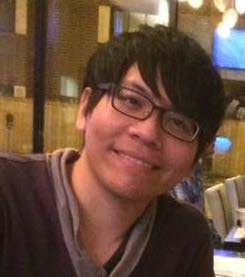
\includegraphics[height=.4\textheight]{chang-tse.jpg} & 
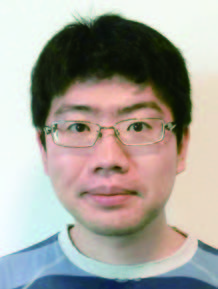
\includegraphics[height=.4\textheight]{kazuya.jpg} \\
Chang-Tse Hsieh & Kazuya Yonekura \\
謝長澤 & 米倉和也 \\ 
\green{cond-mat} & \green{hep-th} \\
IPMU/ISSP & Tohoku
\end{tabular}

\purple{\href{https://dx.doi.org/10.1103/PhysRevLett.123.161601}{PRL123(2019)161601} [\arxiv{1905.08943}] }

\end{center}

\end{frame}

\begin{frame}

I apologize for those who attended my talk at 学習院 last March \\
at 第七回統計物理懇談会, where I gave basically the same talk in Japanese. 

This will be a repeat in English.

The only major change is that at that time only Kazuya (hep-th) was the collaborator, and the paper was unpublished.
To complete it, the help of Chang-Tse (cond-mat) was essential. Now it's a paper with three authors.


\end{frame}


\def\div{\mathop{\mathrm{div}}}
\def\rot{\mathop{\mathrm{rot}}}
\begin{frame}
\LARGE
\begin{align*}
\div \vec B&=0,  &\rot \vec E + \partial_t \vec B&=\vec 0, \\
\div \vec E&=0, & \rot \vec B - \partial_t \vec E&=\vec 0.
\end{align*}
\begin{center}

\bigskip\bigskip

Very important.
\end{center}

\end{frame}

\begin{frame}
\LARGE
\begin{align*}
\div \vec B&=0,  &\rot \vec E + \partial_t \vec B&=\vec 0, \\
\div \vec E&=0, & \rot \vec B - \partial_t \vec E&=\vec 0.
\end{align*}
\begin{center}
Not invariant under the Galilei transformation!

$\downarrow$

It's rather invariant under the Lorentz transformation!
\end{center}

\end{frame}

\begin{frame}
\alert{Anomalies} and \green{topological phases} are closely related.
\[
\incx{pic17e}
\]
Consider the prototypical case of the integer quantum Hall effect:
\begin{itemize}
\item \alert{1+1}d boundary hosts \alert{gapless chiral fermion}
\item \green{2+1}d bulk described by  \green{Chern-Simons}
\end{itemize}
\end{frame}


\begin{frame}
\alert{Anomalies} and \green{topological phases} are closely related.
\[
\incx{pic17e}
\]
Today I consider instead 
\begin{itemize}
\item \alert{3+1}d boundary hosts  \alert{the Maxwell theory}
\item \green{4+1}d bulk described by \green{a cousin of Chern-Simons}
\end{itemize}
\end{frame}


\def\boo#1{{%
\setbeamercolor{background canvas}{bg=myblue!70!black}
\setbeamercolor{author in head/foot}{fg=white, bg=myblue!70!black}
\setbeamercolor{title in head/foot}{fg=white, bg=myblue!70!black}
\setbeamercolor{date in head/foot}{fg=white, bg=myblue!70!black}
\begin{frame}
\vbox{}
\vfill
%\begin{exampleblock}{}
\begin{center}
\bfseries\Huge\color{White} #1
\end{center}
%\end{exampleblock}
\vfill
\vbox{}
\end{frame}
}}

\boo{Electromagnetic duality and  \\[.5em]
Dirac quantization condition}

\begin{frame}
\LARGE\begin{align*}
\div \vec B&=0,  &\rot \vec E + \partial_t \vec B&=\vec 0, \\
\div \vec E&=0, & \rot \vec B - \partial_t \vec E&=\vec 0.
\end{align*}
\begin{center}
Electromagnetic duality: $\vec E\leftrightarrow \vec B$
\end{center}
\end{frame}

\begin{frame}
\LARGE\begin{align*}
\div \vec B&=0,  &\rot \vec E \alert{+} \partial_t \vec B&=\vec 0, \\
\div \vec E&=0, & \rot \vec B \alert{-} \partial_t \vec E&=\vec 0.
\end{align*}
\begin{align*}
S: & (\vec E,\vec B) \mapsto (\alert{-}\vec B,\vec E) \\
S^2: & (\vec E,\vec B) \mapsto \alert{-}(\vec E,\vec B)
\end{align*}
\begin{center}
Although called duality, \\
doing twice is still nontrivial.
\end{center}
\end{frame}


\begin{frame}
\[
\inc{pic1}
\]
\begin{center}
\LARGE
Consider electric charge  $q$ \\
and magnetic charge $m$.
\end{center}
\end{frame}


\begin{frame}
\[
\inc{pic2}
\]
\begin{center}
\LARGE
Poynting vector $\vec E\times \vec B$ gives \\
the angular momentum $\propto qm$.
\end{center}
\end{frame}

\begin{frame}
\[
\inc{pic2}
\]
We fix the units so that \[
\text{anglular momentum} = \frac{\hbar}2 qm.
\] QM demands $qm$ is an integer.

This is the \alert{Dirac quantization condition} (1931).
\end{frame}

\begin{frame}
\[
\inc{pic2}
\]
We haven't chosen the units of charges either.
\[
\text{anglular momentum} = \frac{\hbar}2 qm.
\]
Choose a dimensionless unit such that \\
the smallest charges are $q=1$ and $m=1$.
\end{frame}

\begin{frame}
\[
\inc{pic3}
\]
We can also consider particles with both elec.~and mag.~charges.
\[
\text{angular momentum}=\frac{\hbar}2( \blue{q}\alert{m'}- \blue{m}\alert{q'} ) = \frac{\hbar}2 \det \begin{pmatrix}
q & \alert{q'} \\
m & \alert{m'}
\end{pmatrix}
\]
The transformation \[
\begin{pmatrix}
\vec E \\
\vec B
\end{pmatrix}
\to
\begin{pmatrix}
a & b \\
c & d
\end{pmatrix}
\begin{pmatrix}
\vec E \\
\vec B
\end{pmatrix}
\] acts on $(q,m)$ which are integers. 

So $a,b,c,d$ are also integers.

$\det\begin{pmatrix}
q & q' \\
m & m'
\end{pmatrix}
$ needs to be conserved, so $\det\begin{pmatrix}
a & b\\
c & d
\end{pmatrix}=1$。

\end{frame}
\begin{frame}
\[
\left.
\begin{array}{c}
\text{$a,b,c,d$ are integers} \\[.5em]
\det\begin{pmatrix}
a & b\\
c & d
\end{pmatrix}=1
\end{array}
\right\} \Longleftrightarrow
\begin{pmatrix}
a & b \\
c & d 
\end{pmatrix} \in \alert{SL(2,\mathbb{Z})}
\]
 In particular \[
S: \begin{pmatrix}
\vec E \\
\vec B
\end{pmatrix}
\mapsto
\begin{pmatrix}
-\vec B\\
+\vec E 
\end{pmatrix}
\] comes from  \[
\begin{pmatrix}
a & b\\
c& d
\end{pmatrix}
= \begin{pmatrix}
0 & -1\\
1 & 0
\end{pmatrix}.
\]
\end{frame}

\def\b{\green{b}}
\def\f{\alert{f}}
\begin{frame}
Recall that bosons and fermions have angular momenta
\[
\begin{array}{c|ccccccc}
\text{\green{boson}} & 0\hbar & & \hbar &&2\hbar & &\cdots\\[.5em]
\text{\alert{fermion}} & & \frac{1}2\hbar & & \frac32\hbar && \frac52\hbar & \cdots
\end{array}
\]
So we have
\[
\b+\b=\b; \qquad
\b+\f=\f ;\qquad
\f+\f=\b
\]

\blue{N.B.} I'm relativistic, \\
so the angular momentum determines the statistics.
 
\end{frame}

\begin{frame}
\green{Let's imagine a world where neutral particles are all bosons.}

Then two possibilities:\[
\begin{array}{c|cccccccccc}
\text{elec.~charge}& \cdots & -3 & -2 & -1 & 0 & +1 & +2 & +3 & \cdots \\
\hline
\text{$\b$ or $\f$ ?}& & \b & \b & \b & \b & \b & \b & \b & 
\end{array}
\]or \[
\begin{array}{c|cccccccccc}
\text{elec.~charge}& \cdots & -3 & -2 & -1 & 0 & +1 & +2 & +3 & \cdots \\
\hline
\text{$\b$ or $\f$ ?}& & \f & \b & \f & \b & \f & \b & \f & 
\end{array}
\]
\end{frame}

\begin{frame}
Similarly, there are two possibilities:\[
\begin{array}{c|cccccccccc}
\text{\alert{mag.~charge}}& \cdots & -3 & -2 & -1 & 0 & +1 & +2 & +3 & \cdots \\
\hline
\text{$\b$ or $\f$ ?}& & \b & \b & \b & \b & \b & \b & \b & 
\end{array}
\]or  \[
\begin{array}{c|cccccccccc}
\text{\alert{mag.~charge}}& \cdots & -3 & -2 & -1 & 0 & +1 & +2 & +3 & \cdots \\
\hline
\text{$\b$ or $\f$ ?}& & \f & \b & \f & \b & \f & \b & \f & 
\end{array}
\]

\end{frame}

\begin{frame}
\green{In a world where neutral particles are all bosons,}
there are $2\times 2=4$ slightly different types of Maxwell theories, depending on
\begin{itemize}
\item whether particles with odd elec.~charge is $\b$ or $\f$
\item whether particles with odd mag.~charge  is $\b$ or $\f$
\end{itemize}

\end{frame}

\begin{frame}
How about $\b$/$\f$  of particles with both elec.~and mag.~charges?
\[
\inc{pic4}
\]
Need to recall that there is an additional angular momentum \\
from
  $\frac{\hbar}2 qm = \frac{\hbar}2$. 
  
  
Then, depending on $(q,m)$, we have
\[
\begin{array}{cccccccc}
  (1,0) &+  & (0,1) & \to &  (1,1) \\
 \hline
 \hline
 \b & +&\b & \to &\f \\  
 \b & +&\f & \to &\b \\  
 \f & +&\b & \to &\b \\  
 \hline
 \f & +&\f & \to &\f 
\end{array}
\]
\end{frame}

\begin{frame}
\[
\begin{array}{cccccccc}
  (1,0) &+  & (0,1) & \to &  (1,1) \\
 \hline
 \hline
 \b & +&\b & \to &\f \\  
 \b & +&\f & \to &\b \\  
 \f & +&\b & \to &\b \\  
 \hline
 \f & +&\f & \to &\f 
\end{array}
\]

\bigskip

$SL(2,\mathbb{Z})$ permutes  $(q,m)\equiv (1,0)$, $(0,1)$, $(1,1)$.

\alert{The last one is invariant under  $\alert{SL(2,\mathbb{Z})}$.}

(Sometimes called the all fermion electrodynamics. )

\green{The first three permuted by $\green{SL(2,\mathbb{Z})}$.
Not invariant under $\green{SL(2,\mathbb{Z})}$.}


\end{frame}

\boo{Generalized symmetry and\\[.5em]
the  Maxwell theory }

\begin{frame}
\[
\inc{pic5}
\]
\begin{center}
charged particle in 3d  \quad charged particle in 4d
\end{center}
\end{frame}

\begin{frame}
\[
\inc{pic6}
\]
Symmetry  $g\in G$ in 4d can be visualized as

an operator $\mathcal{O}$ crossing a 3d wall.

Take $G=\mathbb{Z}_2$. If $\mathcal{O}$ is odd,
gets multiplied by $-1$ when crossing the wall.

\end{frame}

\begin{frame}
\[
\incb{pic7}
\]
Can consider ``symmetry'' acting on a line operator,\\
rather than a point operator $\mathcal{O}$.

Captured by a 1d world-line crossing a 2d wall.

\end{frame}

\begin{frame}
\[
\incb{pic7}
\] looks differently depending on how to project it:
\[
\inc{pic8}
\]
\[
\inc{pic9}
\]
\end{frame}

\begin{frame}
Call a ``symmetry'' acting on $p$-dim'l objects a $p$-symmetry.
\[
\begin{array}{cc}
\text{$0$-symmetry} & \inc{pic6} \\[5em]
\text{\alert{$\alert{1}$-symmetry}} & \incb{pic7} 
\end{array}
\]
\end{frame}



\begin{frame}
\[
\incb{pic7}
\]
Maxwell theory has the following two $\mathbb{Z}_2$ \alert{$\alert{1}$-symmetry}:
\begin{itemize}
\item Electric $\mathbb{Z}_2$ \alert{$\alert{1}$-symmetry}:\\
\qquad $(-1)^q$ when crossing a worldline of elec.~charge $q$, 
\item magnetic $\mathbb{Z}_2$  \alert{$\alert{1}$-symmetry}:\\
\qquad $(-1)^m$ when crossing a worldline of mag.~charge $m$
\end{itemize}
Note that the exp.~value of a world-line of elec.~charge $q$ is \\
the Aharanov-Bohm phase $
\exp(2\pi i q\int \vec A \cdot d\vec x ).
$
\end{frame}

\begin{frame}
\begin{gather*}
\incb{pic7}\\
\incb{pic9}
\end{gather*}
$(-1)^q$ when crossing a worldline of elec.~charge $q$.
\end{frame}
\begin{frame}
$(-1)^q$ when crossing a worldline of elec.~charge $q$.
\begin{gather*}
\inc{pic22}\\
\exp(2\pi i q\int_C \vec A \cdot d\vec x )
\mapsto \exp(2\pi i q\int_{C'} \vec A \cdot d\vec x ) \alert{(-1)^q }
\end{gather*} 
This means that the black wall realizing the electric $\mathbb{Z}_2$  \alert{$\alert{1}$-symmetry}  has\\
\alert{half the flux} of the magnetic quantum  \[
\vec B=\oint  \vec A \cdot d\vec x  
= \int_C  \vec A \cdot d\vec x -\int_{C'}  \vec A \cdot d\vec x 
=  \pm\frac12
\]

\end{frame}

\begin{frame}
\[
\incb{pic10}
\]
$(-1)^m$ when crossing a worldline of mag.~charge $m$.
\end{frame}

\begin{frame}

$(-1)^m$ when crossing a worldline of mag.~charge $m$.
\[
\incb{pic23}
\]
This means that the green wall realizing the magnetic $\mathbb{Z}_2$  \alert{$\alert{1}$-symmetry}  has the factor \[
\exp(\pi i \iint \vec B \cdot d\vec\sigma)
\]
\end{frame}

\begin{frame}
\begin{gather*}
\text{Wall for elec.~$\mathbb{Z}_2$ \alert{$\alert{1}$-symmetry}
 \qquad Wall for mag.~ $\mathbb{Z}_2$ \alert{$\alert{1}$-symmetry}}\\
\qquad\qquad\vec B= \pm\frac12 \qquad\qquad \exp(\pi i \iint \vec B \cdot d\vec\sigma)\\[-2em]
\incb{pic11}
\end{gather*}
Problematic if  both are inserted  at the same time,\\
since two 2d surfaces intersects at points in 4d.
\[
\inc{pic12}
\]
\end{frame}

\begin{frame}
If depicted in one lower dimension,\[
\inc{pic13}
\]
You can't tell if the phase is  which of  \[
e^{\pm\pi i/2} =\pm i
\] 
\end{frame}

\begin{frame}
An \alert{anomaly} is when the phase of the partition function and the expectation values
become ambiguous in a quantum field theory.

Originally found concerning the $U(1)$ symmetry of chiral fermions \\
in the late 60s.

What I described so far is the mixed anomaly \\
of elec.~$\mathbb{Z}_2$ \alert{$\alert{1}$-symmetry} and mag.~$\mathbb{Z}_2$ \alert{$\alert{1}$-symmetry}.
\end{frame}

\boo{Global Gravitational Anomaly \\[.5em]
of the Maxwell theory}

\begin{frame}
Let's combine the two stories together.

In 3+1d, rotating $720^\circ$ is trivial, while 
rotating $360^\circ$ is nontrivial.

Something is a fermion if $360^\circ$ gives you $-1$: \[
\incb{pic14}
\]

\end{frame}

\begin{frame}
Particles with elec.~charge $q=1$ are fermions \\
$\leftrightarrow$ twisting by $360^\circ$ is
equal to \\
surrounding by a wall for elec.~$\mathbb{Z}_2$  \alert{$\alert{1}$-symmetry}
\[
\incb{pic15}
\]
\end{frame}

\begin{frame}
Particles with mag.~charge $m=1$ are fermions \\
$\leftrightarrow$ twisting by $360^\circ$ is
equal to\\
 surrounding by a wall for mag.~$\mathbb{Z}_2$  \alert{$\alert{1}$-symmetry}
\[
\incb{pic16}
\]
\end{frame}

\begin{frame}

You can't say you don't care about twisting particles!

When 3+1d spacetime  is nontrivial, the pasting together coordinate patches can produce twisting by $360^\circ$.

This is measured by the \green{Stiefel-Whitney class} $w_2$, \\
introduced in math in the 1940s.

They are  $\mathbb{Z}_2$ walls of representing $360^\circ$ twists, \\
intrinsically present in 3+1d spacetime $M_4$. 

%複素射影平面 $\mathbb{CP}^2$ だと、$w_2$ はその中の複素射影直線 \[
%w_2=\mathbb{CP}^1\subset \mathbb{CP}^2
%\] に対応。


\end{frame}

\begin{frame}
Now recall the four versions of the Maxwell theory:

\[
\begin{array}{c|ccccccc}
(q,m) &  (1,0)  & (0,1) &   (1,1) \\
 \hline
 \hline
& \b & \b & \f \\  
& \b & \f & \b \\  
& \f & \b & \b \\  
 \hline
& \f & \f & \f 
\end{array}
\]

\bigskip

$SL(2,\mathbb{Z})$ exchanges $(q,m)\equiv (1,0)$, $(0,1)$, $(1,1)$.

The last one is invariant under  $SL(2,\mathbb{Z})$.

The first three are permuted by $SL(2,\mathbb{Z})$.

\end{frame}

\begin{frame}
\[
\begin{array}{c|ccccccc}
(q,m) &  (1,0)  & (0,1) &   (1,1) \\
 \hline
 \hline
& \b & \b & \f \\  
& \b & \f & \b \\  
& \f & \b & \b \\  
 \hline
& \f & \f & \f 
\end{array}
\]

The first three $SL(2,\mathbb{Z})$ non-invariant have \green{no issues}:\\
You \green{never insert both} walls for elec.~$\mathbb{Z}_2$  \alert{$\alert{1}$-symmetry}\\
and walls for mag.~$\mathbb{Z}_2$ \alert{$\alert{1}$-symmetry}.

The last $SL(2,\mathbb{Z})$ invariant one has \green{a problem}:\\
\green{Need to insert both} walls for elec.~$\mathbb{Z}_2$  \alert{$\alert{1}$-symmetry}\\
and walls for mag.~$\mathbb{Z}_2$ \alert{$\alert{1}$-symmetry}.

The partition function can be ambiguous by $\pm1$.

\end{frame}

\begin{frame}
\[
\begin{array}{c|ccccccc}
(q,m) &  (1,0)  & (0,1) &   (1,1) \\
 \hline \hline
& \f & \f & \f 
\end{array}
\]

For example, on the complex projective space $\mathbb{CP}^2$,\\
to account for $360^\circ$ twists,\\
we need to put  walls for 
both elec.~$\mathbb{Z}_2$ \alert{$\alert{1}$-sym.} and mag.~$\mathbb{Z}_2$ \alert{$\alert{1}$-sym}  \\
at $w_2=\mathbb{CP}^1\subset \mathbb{CP}^2$.

\end{frame}

\begin{frame}
Two  $\mathbb{CP}^1$ within $\mathbb{CP}^2$ intersect at one point:
\[
\inc{pic13}
\]
producing a $\pm1$ ambiguity.

For example, a global coordinate transformation 
$[z:w] \mapsto [\bar z:\bar w]$ \\
of $\mathbb{CP}^2$
flips the sign of the partition function.

\end{frame}

\begin{frame}
Summarizing, the  $SL(2,\mathbb{Z})$-invariant Maxwell theory with \[
\begin{array}{c|ccccccc}
(q,m) &  (1,0)  & (0,1) &   (1,1) \\
 \hline \hline
& \f & \f & \f 
\end{array}
\]
has a \alert{subtle breaking of general covariance}.

This is an example of a \alert{global gravitational anomaly}.

\loosecite{Wang-Wen-Witten \arxiv{1810.00844}}

\end{frame}

\boo{Maxwell theory as living\\[.5em]
on the boundary}

\begin{frame}
\alert{Anomalies} and \green{topological phases} are closely related.
\[
\incx{pic17e}
\]
The phase ambiguity of the boundary partition function is canceled against
the   phase ambiguity of the bulk partition function.
\end{frame}


\begin{frame}[label=inflow]
\alert{Anomalies} and \green{topological phases} are closely related.
\[
\incx{pic17e}
\]
The prototypical case is the integer quantum Hall effect: \hyperlink{detail}{\beamerbutton{details}}
\begin{itemize}
\item \alert{1+1}d boundary hosts \alert{gapless chiral fermion}
\item \green{2+1}d bulk described by  \green{Chern-Simons}
\end{itemize}
\end{frame}


\begin{frame}
\alert{Anomalies} and \green{topological phases} are closely related.
\[
\incx{pic17e}
\]
Today I consider instead 
\begin{itemize}
\item \alert{3+1}d boundary hosts  \alert{the Maxwell theory}
\item \green{4+1}d bulk described by \green{a cousin of Chern-Simons}
\end{itemize}
\end{frame}

\def\Sq{\mathop{\mathrm{Sq}}\nolimits}
\begin{frame}
For 
elec.~$\mathbb{Z}_2$ \alert{$\alert{1}$-symmetry} and
mag.~$\mathbb{Z}_2$ \alert{$\alert{1}$-symmetry},
we introduce background fields  \[
A_\text{e}, A_\text{m} \in H^2(M_5,\mathbb{Z}_2).
\]The bulk ``Chern-Simons'' action is  \[
\exp(\pi i \int_{M_5} A_\text{e} \alert{\Sq^1} A_\text{m})
\]
where  $\Sq^1$ is one of the  \green{Steenrod squaring operation}\\
(which is introduced in 1940s in algebraic topology)

You might be scared of these expressions, but recall that
the Chern-Simons action, introduced in mid-1970s, is \[
\exp( \frac{ i k}{4\pi}   \int_{M_3} AdA )
\] and they look similar. 



\end{frame}

\begin{frame}
For the anomaly under general covariance,
we take both $A_\text{e}, A_\text{m}$ to be the 
\green{Stiefel-Whitney class} $w_2$. Then the bulk action is \begin{align*}
\exp(\pi i \int_{M_5} A_\text{e} \alert{\Sq^1} A_\text{m})
&=\exp(\pi i \int_{M_5} w_2 \alert{\Sq^1} w_2) \\
&= \exp(\pi i \int_{M_5} w_2  w_3) .
\end{align*}
known as the 
\green{de Rham invariant}.

(This invariant was introduced in 1931.
The expression in terms of Stiefel-Whitney class came slightly later)
\end{frame}

\begin{frame}
When two oriented manifolds $M_d$, $M_{d}'$ are connected by $X_{d+1}$ ,
\[
\inc{pic19}
\]
they are called bordant: $M_d\sim M_d'$.

The equivalence class is the bordism class.

\end{frame}

\begin{frame}
\[
\inc{pic19}\qquad \inc{pic20}
\]
There are only two oriented bordism classes in 5d, and distinguished by
de Rham invariant: \[
\exp(\pi i \int_{M_5} w_2  w_3) = \pm1 
\] 

You can shrink $M_5$ if $+1$;
you can't if $-1$.

\end{frame}

\begin{frame}
These are results of algebraic topology in the 1950s and 1960s.\\
Chern-Simons was introduced in the mid-1970s, \\
so these are older stories and should be easier.

In mathematical physics we use various subfields of math.\\
But \green{we haven't used much algebraic topology}.

It's interesting that we now use \green{algebraic topology from 50 years ago}, \\
and that \green{this trend started from mathematical condensed-matter theory}.

\end{frame}

\boo{The relation to our work}

\begin{frame}

So far I only talked about known stories, on which our work is based.

With Chang-Tse Hsieh (謝長澤) and Kazuya Yonekura (米倉和也),\\
we determined the anomaly of the electromagnetic duality of the Maxwell theory.

Thanks to the bulk-boundary correspondence, \\
all have to do is to analyze
the 4+1d bulk Chern-Simons-like theory.\\
It's somewhat complicated but it can be done.

We found that the anomaly is $56$ times that of a fermion.

Why $56$? 

It's the dimension of the smallest nontrivial representation of $E_7$,\\
one of the exceptional Lie group.

\end{frame}

\begin{frame}

The point is that the 3+1d Maxwell theory is a $T^2$ compactification of a 5+1d self-dual tensor theory.

This self-dual tensor theory can be embedded into the tensor branch of the E-string theory, which is a superconformal field theory with $E_8$ symmetry.
The E-string theory also has the Higgs branch, to which we can go continuously.
\[
\incb{pic21e}
\]
On the Higgs branch, $E_8$ is broken to $E_7$, leaving $56$ fermions.

\end{frame}

\begin{frame}
\[
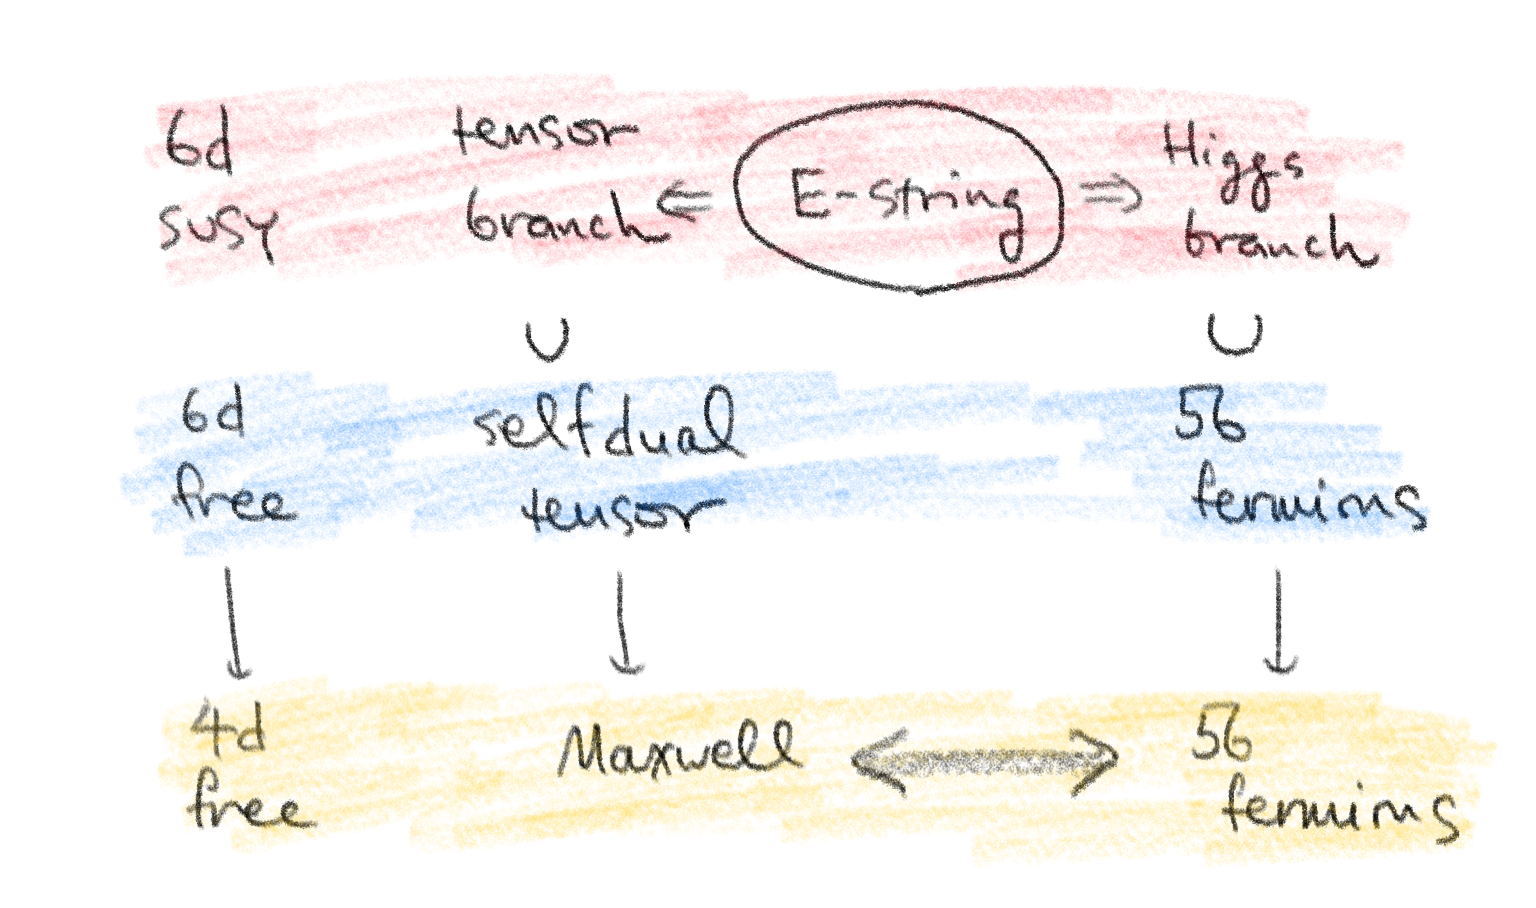
\includegraphics[width=1\textwidth]{pic24e}
\]
\end{frame}

\begin{frame}
The E-string theory is the smallest nontrivial 5+1d superconformal theory,
and Kazuya and I were studying this from a totally different motivation for about six years.

Somehow it turned out to be `useful' to understand a subtle feature of 3+1d Maxwell theory.
This pleasantly surprised me.

I'd like to emphasize, though, that \green{the analysis can be and was first done purely field theoretically, without invoking string theory.}
It's just that string theory provides a quicker, more conceptual derivation, if you happened to know string theory already.

We already have a short letter \loosecite{\arxiv{1905.08943}}.
We're preparing a longer version to fill in the detail.
Please have a look if you're interested.

\end{frame}

\boo{ Supplement:  anomaly on the \\[.5em]
boundary of  Chern-Simons }

\begin{frame}[label=detail]
Consider the electromagnetic $U(1)$.
The gauge transformation is  \[
 A_\mu \to  A_\mu+\frac{1}{2\pi i} e^{-2\pi i\chi}\partial_\mu  e^{2\pi i\chi} = A_\mu + \partial_\mu \chi
\] 
so we have \[
\oint A_t dt \to \oint A_t dt + \oint \partial_t \chi dt 
\] Note that $\chi\sim \chi+1$ so we need to identify  \[
\oint A_t dt \sim \oint A_t dt + 1.
\]
\end{frame}


\begin{frame}
Consider a $1+1$d fermion on a circle:
\[
\inc{pic18}
\]
Energy levels of one particle states are  \[
E \propto n + \oint A_t dt
\]
The negative energy states are filled;
this is the Dirac sea.
\end{frame}
\begin{frame}
A careful regularization shows that the Dirac sea has the electric charge \[
\green{q = \oint A_t dt }.
\] 
The partition function is \[
Z=\tr e^{-\beta H} e^{ i\green{q} \alert{\oint A_t dt}}
\] which varies under the gauge transformation\[
\alert{\oint A_t dt} \to \alert{\oint A_t dt }+\alert{\oint \partial_t \chi dt}
\] as \[
Z \to Z e^{i\green{q}\alert{\oint \partial_t \chi dt}} = Z \exp({i\alert{\oint \partial_t \chi dt}\green{\oint A_t dt}}).
\] The phase of the partition function is ambiguous!
\end{frame}


\begin{frame}
The bulk effective action is the Chern-Simons term $e^{iS_\text{CS}}$ where \[
S_\text{CS}=\int_{M_3} AdA \propto \int_{M_3} \epsilon^{\mu\nu\rho} A_{\mu} \partial_\rho A_\sigma
\]
The gauge transformation  \[
A\mapsto A+d\chi
\] changes it by \[
\delta \int_{M_3} AdA = \int_{M_3} d\chi dA 
= \int_{\partial M_3} (d\chi) A
\]
which becomes  \[
= \oint \alert{\partial_t\chi dt} \oint \green{A_x dx},
\]  cancelling the phase ambiguity  of the 1+1d fermion on the boundary.

\hyperlink{inflow}{\beamerbutton{Back}}
\end{frame}

\end{document}
